\documentclass[conference]{IEEEtran}
\IEEEoverridecommandlockouts
% The preceding line is only needed to identify funding in the first footnote. If that is unneeded, please comment it out.
\usepackage{cite}
\usepackage{amsmath,amssymb,amsfonts}
\usepackage{algorithmic}
\usepackage{graphicx}
\usepackage{textcomp}
\usepackage{xcolor}
\usepackage{array}
\usepackage{soul}
\def\BibTeX{{\rm B\kern-.05em{\sc i\kern-.025em b}\kern-.08em
    T\kern-.1667em\lower.7ex\hbox{E}\kern-.125emX}}
\begin{document}

\title{{Secure Privacy Preserving Deep Learning against GAN attacks}\\
\author{\IEEEauthorblockN{Aseem Prashar}
\IEEEauthorblockA{\textit{Department of Electrical Engineering and Computer Science} \\
\textit{Wichita State University}\\
Wichita, USA \\
prasharaseem@gmail.com}
\and
\IEEEauthorblockN{Sergio A. Salinas Monroy}
\IEEEauthorblockA{\textit{Department of Electrical Engineering and Computer Science} \\
\textit{Wichita State University}\\
Wichita, USA \\
sergio.salinasmonroy@wichita.edu}
}
}
\maketitle

\begin{abstract} 

%Deep learning is a class of machine learning algorithms that use a cascade of multiple layers of non-linear processing units to
%perform statistical inferences. 
Deep neural networks are becoming increasingly popular in a variety of fields due to their ability to learn from large-scale data sets.
%. Deep neural networks benefit from larger input data sets and can be
%revolutionary to organizations that have access to sizeable rawdata. 
Recently,  researchers have proposed distributed learning architectures that allow multiple
users to share their data to train deep learning models. Unfortunately, privacy and confidentiality concerns limit the application of
this approach, preventing certain organizations such as medical institutions to fully benefit from distributed deep learning.  To
overcome this challenge, researches have proposed algorithms that only share neural network parameters. This approach allows 
users to keep their private datasets secret while still having access to the improved deep neural networks trained with the data from
all participants. However, existing distributed learning approaches are vulnerable to attacks where a malicious user can use the
the shared neural network parameters to recreate the private data from other users. 
%Other existing research uses computationally
%expensive cryptographic i

To overcome this challenge, we propose a distributed deep learning algorithm that allows a user to improve its
deep-learning model while preserving its privacy from such attacks. 
Specifically, 
%we design our approach to protect organizational data against attacks that involve a malicious participant that can learn
%meaningful information from the abstracted dataset. 
our approach focuses on protecting the privacy of a single user by limiting the number of times other users can download and upload
parameters from the main deep neural network. By doing so, our approach limits ability of the attackers to recreate private data
samples from the reference user while maintaining a highly accurate deep neural network. 
%Our solution does not involve computationally expensive cryptographic processes and relies on limiting the exposure of private dataset
%of participants. 
Our approach is flexible and can be adapted to work with any deep neural network architectures. We conduct extensive experiments to
verify the proposed approach. We observe that the trained neural network can achieve an accuracy of 95.18\%, while protecting the privacy
of the reference user by preventing it from sharing both its private data and deep neural network parameters with the server or other
users.
\end{abstract}

\begin{IEEEkeywords}
Neural Network, Deep learning, GANs
\end{IEEEkeywords}

%---------------------------------------------------------------------------------
\section{Introduction}
%---------------------------------------------------------------------------------
In the past few decades, deep learning has generated a lot of interest in the research and academic community due to its great ability
to automatically classify large amounts of data. This has led to breakthroughs in many fields ranging
from autonomous driving, and natural language processing to genetic research 
\cite{young2018recent, al2017deep, huval2015empirical, danaee2017deep}.
%It is no surprise that deep learning has seen a significant investment by technology giants such as Google, IBM and Facebook. 
This revolutionary technology is especially fruitful for large corporations that need to automatically process very large data sets to
provide deep learning inference services to their users. For example, data collection at Facebook enabled them to create DeepText, a
text understanding engine that is able to extract meaningful context from text \cite{abdulkader2016introducing}.

Although it is possible to collect large-scale data to train deep learning models in some application domains, e.g., online social
networks, there are other fields where such centralized data collection is currently infeasible due to privacy
concerns. In particular, users' data can contain instances of private information that needs to be kept a secret from third-parties
such as the companies that centrally collect data to provide deep learning services. Such data
can include
%It is only inevitable that a
%subset of the sample space contains sensitive information that was accidentally captured without user consent.  Other privacy concerns
%regarding data ownership have also been raised since the trained model is generally a 
intellectual property (IP), 
%. Other %red flags are centered around 
medical data protected by Health Insurance and Portability and Accountability Act (HIPA), and student records protected by the Family
Educational Rights and Privacy Act (FERPA) \cite{act1996health,blechner2002health,shultz2015your}. 
%While medical
% community
%By sharing their data, organization can receive improved deep learning inference. However, 
%stands to benefit from deep learning, 
%the privacy concerns around these type of data make it impossible to share with an untrusted third-party such as a deep learning
%service provider. 
%medical history of patients makes collecting of data samples a challenging task. 

Instead of sharing private data with a third-party, users could locally train their own deep learning models using their own
data. However, since a single user only has access to a small data set compared to the data set that could be centrally
collected by the third-party, its locally trained deep learning model have low accuracy, which
significantly degrades its ability to provide correct inferences. 
Moreover, locally trained models can suffer from over generalization can prevent them from being used in practical scenarios.
For instance, a hospital trained a deep neural network to recognize patients with pneumonia based on their
chest X-ray images using its own records. Although this neural network was successful in classifying records from patients that were
treated in this hospital, its performance significantly dropped when tested with images from other patient treated at a different
hospital \cite{zech2018variable}. This was due to the fact the trained deep neural network was basing its inferences on the
particular imaging machine used at the hospital  rather than on the the content of the image itself.
%This indicates that models trained on single source datasets can produce confounding results. 
%Moreover, many organizations may not have large enough local data sets to train a deep learning model with satisfactory
%accuracy. 
%Accessibility of training datasets in hospital that do not have sufficient resources or samples currently is also a concern.
 
The above outlined issues beg for a deep learning solution that can achieve high accuracy while preserving privacy. 
Researchers have made some headway in this direction by leveraging distributed learning.
In this approach  \cite{shokri2015privacy},  a set of users locally
train a deep learning model only using their local data. To overcome the challenge of over generalization and small
data sets, they send certain parameters of their model to a central server for aggregation. 
Then, the users can download the aggregated parameters to improve their local models. This approach achieves high accuracy.
Although users can protect their private data by only sharing the model parameters, recent studies have
shown that it is possible for malicious users to recreate samples of other users by using a generative
adversarial network (GAN) \cite{hitaj2017deep}. This attack can be successful even when the victim users 
obfuscated their private data before performing  local training. 

In this paper, we design, implement, and analyze a distributed deep learning framework that enables a user 
to benefit from highly accurate distributed learning while preserving the privacy of its local data. 
%and the privacy of all other users. 
Specifically,  instead of attempting to protect the privacy of all users as in \cite{shokri2015privacy}, we focus on protecting the
privacy of a single user, called the reference user, by preventing it from uploading its model's parameters to the server. Hence,
other malicious users are unable to launch the attack describe in \cite{hitaj2017deep} against the reference user. To further limit the
ability of a malicious user to launch attacks, the parameter server only accepts parameters from randomly
selected users at each iteration, which significantly decreases the accuracy of the GAN attack described in \cite{hitaj2017deep}. 

Our framework operates as follows. First, all users train a local deep learning model using only their local data.
Second, the framework randomly selects a set of users to upload their parameters to be aggregated by the server. The reference user is
never selected. Third, the reference user and the selected users download the aggregated parameters and update their local
deep learning models. The iteration continues until the reference user's deep learning model achieves a minimum
accuracy, or a maximum number of iterations is reached.

The main contribution of our approach is that it allows the main user to leverage the data sets form the other users to train a local
deep learning model with high accuracy while protecting its private data from the parameter server, and other users who
may launch sophisticated GAN based attacks as described in \cite{hitaj2017deep}. The proposed architecture is independent of the
neural network architecture of the system, and is therefore, adaptable to any deep neural network. Our proposed privacy-preserving
distributed learning approach can potentially be used in a scenario where the privacy of one of the participant in distributed learning is valued over other participants. For instance, a medical facility that has classified medical data can still benefit from distributed deep learning using our approach. 

% We accomplish this by a two pronged approach.
% First, we randomly select users that can upload and download parameters from the server at each iteration. This prevents the
% attacks in \cite{hitaj2017deep} by limiting the repeated and predictable exposure of potential victims to the malicious users.
% Second, we enable a user with insufficient but extremely sensitive sample set to benefit from the architecture, while completely
% safeguarding itself from GAN based attacks. 

To verify the efficacy of our approach, we implement it using a multilayer perceptron (MLP), and the scripting language
LUAJIT. We run our experimental simulation on an M4 instance on the Amazon Web Service's Elastic Compute Cloud (AWS EC2). 
The MLP is trained to  classify images from the MNIST dataset, which is a benchmark dataset,  for image classification.
We observe that our approach can achieve up to 95.18\%  accuracy for the main user when there are 20 other users in the
system with each one having 50\% probability of being selected to upload their parameters at each iteration. 
%In comparison, the accuracy when all participants were selected, was 95.17\% with other comparable variables. 
This is a comparable accuracy to the one that can be achieved by running a non-privacy-preserving centralized approach, i.e.,  98.17\%.
%The privacy violating centralized architecture with comparable variables yields an accuracy of 98.17\%. 
%We achieve these results without deploying any additional computationally intensive obfuscation or cryptographic techniques. 
We also measure the trade-off between privacy and accuracy, and show that the main user can easily choose the most appropriate
trade-off by tuning the user selection probability. 


%---------------------------------------------------------------------------------
\section{Related Work}
%---------------------------------------------------------------------------------

Deep neural networks have outperformed traditional machine learning approaches for many tasks, and are the tool of choice in many
fields. Specifically, Deep learning has been successfully used for facial recognition \cite{krizhevsky2012imagenet, sun2014deep, ding2015robust}, image classification, 
\cite{simard2003best, ma2015hyperspectral, zhong2011bilinear}, and speech recognition \cite{hinton2012deep, graves2013speech, noda2015audio}, where it is expected to achieve better
performance than humans in the near future. However, directly applying these techniques in fields that deal with private data is
challenging. The reason is that they need to centrally collect data at a third-party which organizations may not trust
\cite{chicurel2000databasing}. This is particularly challenging in medical and financial applications where the privacy of the users is
governed by federal legislation and is protected by law. 

% This has however raised some privacy issues.

To protect users' data privacy, some researchers have proposed to use secure multiparty computations (SMC) 
\cite{vaidya2003leveraging,7040943, ma2018privacy}. 
SMC is a cryptographic technique used to distribute computation over many parties while preserving each party's privacy. It allows
users to securely and privately compute encrypted data distributed across users. 
%In , the authors survey multi party computation as well as other techniques. They also evaluate SMC's effectiveness and
%cost in context of secure data processing.
Sheikh et al. \cite{sheikh2010distributed} propose a SMC that divides and distributes private data blocks among participants and can
prevent the participants from learning the data from  each other. This approach assumes a semi-honest threat model,
where a malicious  participant attempts to learn the private from other users but does not deviate from the proposed
protocol. 
%datahonest parties are incapable of discovering private data of other parties. This technique is however contingent
%on the malicious
%parties being semi-honest parties.
Miyajima et al. \cite{miyajima2016new} propose a back propagation learning method for secure data computation and learning on a cloud
based system using SMC. %solve security risks associated with cloud computing using SMC. 
Bonawitz et al. \cite{bonawitz2017practical}  proposed an SMC protocol to aggregate mobile user data that maintains its efficacy even
if there are some users who dropout of the system.  Unfortunately, SMC is computationally expensive for the users participating in the
system, which can be impractical for mobile users or IoT devices. Moreover, SMC reveals the result of the computation to all parties,
which may be a privacy risk for certain applications. 

%d
%To overcome constraints in a mobile user setting, some researchers haveby leveraging SMC
%. They focus their work on creating a robust protocol 

Differential privacy has also been proposed to protect users' data privacy  in distributed deep learning
\cite{vepakomma2018no}. 
In Abadi et al. \cite{abadi2016deep} propose a novel differential privacy algorithm to training deep neural networks with a modest
accuracy cost and a feasible computational complexity. They provide theoretical analysis of the the privacy cost, complexity and
training efficiency of their proposed approach. 
%neural networks where users employ
%differential privacy to hide their information. They Their work however does not account for distributive collaborative deep learning.
%jthe added noise will scale with size
%of the participants. Ultimately, the amount of noise added will render the shared data to have no
%practical use.
Song et al. \cite{song2013stochastic} investigate effects of differential privacy on mini batch SGD. They observe that increased batch
size ameliorates the impact of differential privacy on the variability of SGD. 
%The authors, however, also observe an upper limit to the
%batch that can be utilized to control the variability produced by the privacy preserving noise.
Chase et al. \cite{chase2017private} propose an algorithm that combines  SMC and differential privacy. 
Unfortunately, since differential privacy adds noise to the private data, the accuracy degradation increases with the number of users
in the system. Hence, differential privacy approaches suffer from poor scalability. 

To protect the privacy of the users while allowing a large amount of users to participate in training of deep learning
models, researchers have recently proposed distributed learning. Specifically, Shokri et al. \cite{shokri2015privacy} propose 
%a  system that enables collaborative training for deep neural networks in a privacy
%preserving manner. In the paper the authors design and test 
a protocol where the users locally train a deep neural network and then share a small subset of its parameters
with a server. The server aggregates the users' parameters, and then the users choose which parameters to download. 
Using the downloaded the parameters, the users can improve their deep learning models without having to observe the data sets from the
other users, which preserves their privacy. Under this approach, the users are able to train their models to a high accuracy. 
%uploads  enables %the participants to preserve the privacy of %their dataset while drawing benefits from other participants' trained model.

Unfortunately, the privacy-preserving distributed learning proposed by Shokri et al. \cite{shokri2015privacy} is vulnerable to an
attack where users upload maliciously crafted parameters. Specifically, Hitaj  et al. \cite{hitaj2017deep} design
an attack where a malicious user 
%exploits the architectural weaknesses in distributed learning. 
%system proposed in \cite{abadi2016deep}. 
%The attack proposed in \cite{hitaj2017deep} 
leverages Generative Adversarial Networks (GAN) to replicate samples of the data sets from other users in the system, which compromises
their privacy. \hl{[Ideally, we would have one or two sentences explaining how the attack is launched here. ]} 
%their attack model immune to majority of obfuscation techniques. 


%---------------------------------------------------------------------------------
\section{Deep Neural Networks}
%---------------------------------------------------------------------------------
Deep neural networks are a type of machine learning that has recently shown high accuracy in data classification tasks. Traditional
machine learning requires manual feature selection, which can be time consuming and inaccurate. In contrast, deep learning
learns the most relevant features in the data on its own. In other words, the deep neural networks can be trained with raw data without
the burden of preprocessing it. Since deep neural networks have more hidden layers compared to traditional neural networks, their
accuracy is proportional to the amount of data used for training, i.e., the larger the training data set the more accurate that the
deep neural networks become. These advantages make deep neural networks a very effective technique to perform data classification
tasks. In this section, we describe the architecture of deep neural networks and their training methods. 

%The layers of deep neural networks can be of three types: input, hidden or output. 

%------------------------------------------------------------------------------
\subsection{Architecture}\label{sec:MLP}
%------------------------------------------------------------------------------
%the network, process it, and provides an input to the first hidden later. Hidden layers continue the data flow until they reach
%the output layer, which provides the results of the classification task to the user. 
%Deep neural networks contain two or more hidden layers. The large number of hidden layers enable deep neural networks to
%learn nonlinear relationships between the input and the output, making them powerful tools for many tasks beyond classification. 

\begin{figure*}[t]
\centering
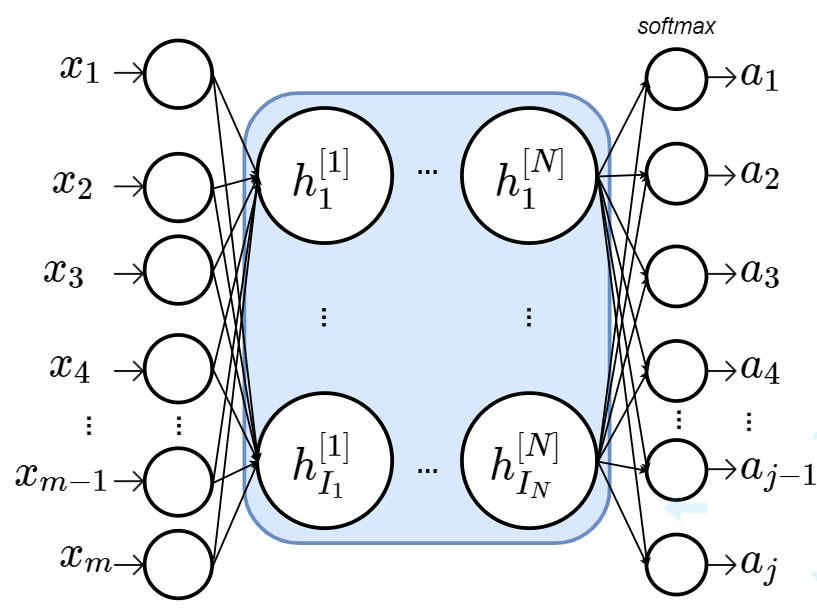
\includegraphics[width=0.5\textwidth, keepaspectratio]{SimpleNN}
\caption{A neural network with $m$ inputs, $j$ outputs,  $N$  hidden layers, and $I$ neurons per layer.}
\label{fig:SimplNN}
\end{figure*}
One of the most common deep learning architectures is the multilayer perception (MLP). 
An MLP is formed by input, hidden, and output layers where each layer consists of many nodes. Each node takes 
as input a weighted average of the previous layer's node outputs, and the output of an special node called the bias.  
The nodes use a non-linear activation function to the compute their output. Together, the weights used in the weighted average and
the biases from the special neurons are called the parameters of the deep neural network. 
For ease of exposition, we focus on MLP. However, our results and formulations are generalizable to any deep neural network
architecture. 

% from nodes in the
% previous layer.The layers are sequentially connected to
% each other by 
% previous one and the next layer in the architecture. The output of a node
% within a layer is a function of the weighted averages of the outputs from nodes in the previous layer. Each node also receives an
% additional input from a special neuron called the bias.  
% %The weighted average of inputs plus the bias is referred to as the total input for the
% %neuron. 

%This activation
%function is crucial in introducing non-linearity in neural networks. The non-linearity allows the modeling of complex relationships
%between the input and the outpout data. 

%a a feed-forward based network, i.e., it has no feedback loops, The MLP architecture 

Figure \ref{fig:SimplNN} shows the structure of a typical classification MLP with $m$ input nodes and $j$ outputs nodes. The neural network
has $N$ hidden layers and each layer has $I$ neurons. Intuitively, this MLP takes a data sample represented as a vector of length
$m$ on its input layer, and outputs the probability that it belongs to the $j$th category on the $j$th output neuron.
Formally, the output of the $i$th neuron at layer $k$ is defined as follows:
$$a^i_k=f(W_k a_{k-1}),$$
where $f$ is the activation function, $W_k$ is the weight matrix of layer $k$,
%which controls how input signal from previous layer,
and $a_{k-1}$ is the vector of neuron outputs from the the $k-1$th layer. 
%affects the output of the current neuron. 

There are several non-linear activation functions that can be used for function $f$, including sigmoid,
hyperbolic tangent, and rectified linear unite (ReLU) \cite{Goodfellow-et-al-2016}. In this
work, we will focus on the ReLU activation function:
$$f(z) = \max\{0, z\},$$
where given an input $z$ the function returns $z$ for positive values and $0$ for negative values.
%function which outputs
%values between 0 and 1, normalizing the output of each neuron. Hyperbolic tangent activation function 
%is zero centered and makes it easier to model inputs that have strongly negative, neutral or positive values. 
%Rectified Linear Unit (ReLU) is an increasing popular activation function that aids in the quick convergence of the network. 

%In a network that is tasked to classify inputs to one of the $j$ fixed number of outputs, 
The output layer is usually implemented with the SoftMax activation function. The output of this function is between zero and
one, and it is used to the output of the last hidden layer to a scalar that represents the probability that the data sample observed at
the input layer belongs to each of the $j$ categories. Formally, the SoftMax activation functions is defined by
%divides it by their sum, resulting in a probability
%score that
%the given input belongs to class $j$. which is given by
$$f(z)_j = \frac{e^{z_j}} {(\sum_ke^{z_k})} \ \  \forall j,$$
where $z_j$ is the $j$th element of the input vector $z$ with $k$ elements (e.g., the output of all the neurons in the last hidden
layer).
% and  and $\sum_k e^{z_k}$ is sum of exponents of all elements in
%$z$.

%---------------------------------------------------------------------
\subsection{Training}
%---------------------------------------------------------------------
Before a neural network can be used to perform inference, e.g., classify images, it needs to be trained to learn the highly non-linear relationships between the inputs and the correct outputs. Training finds the
parameters of the deep neural network, i.e., its the weights and biases, that result in the inferences with the highest accuracy.  

Although there are many training algorithms, their general workflow is the same. 
First, we randomly initialize the deep neural network parameters.
Then, we take a data sample from the training data set, e.g., an image, and feed it as input to the deep neural network. Based on the
inference error, e.g., the difference between the probability given by the neural network that the image belongs to certain category
and the correct probability, we adjust the value of the parameters in such a way that the inference error is reduced. This iteration is
repeated until the inference error converges or a maximum number of iterations is reached. 


%There are several algorithms that can tackle this non-linear optimization problem. A training dataset is a dataset of sample
%inputs which has  known outputs or labels. In supervised learning,  we feed the inputs from a training dataset to the neural network
%during its training phase and compare computed output with the corresponding labels.

The main challenge in training is finding a parameter update at each iteration that drives the deep neural network to the optimal
classification accuracy. The most common way of finding these updates is by using the gradient descent (GD) algorithm, or one of its
variants. In the rest of this subsection, we provide a brief overview of these algorithms. 

%---------------------------------------------------------------------
\subsubsection{Gradient Descent Algorithm}
%---------------------------------------------------------------------
The GD algorithm finds the parameter updates in two steps: forward propagation and back propagation. 
 %calculates the parameter update at each iteration by performing forward
%propagation, and then updates the parameters through
%backward propagation. 

In the forward propagation step, the GD algorithm passes the samples in its training data set through the
deep neural network and obtains the output for each sample based on the current value of its parameters. Then, the GD computes the
error function, which measures the difference between the outputs of the neural network and the correct classification solutions,
which we call labels. There are multiple ways of calculating the error. In this work, we focus on the mean squared error function,
which is defined as follows:
\begin{align}\label{eq:errorFunction}
 E= \frac{1}{n} \sum_{n=1}^{n}(y_i -\hat{y_i}),
\end{align}
where $n$ is the the number of samples in the training dataset, $y_i$ is the output calculated by the neural network and 
$\hat{y_i}$ is the correct label for the $i$th sample.


%The error is given by the difference between the label of the training set and the computed output by the neural network. 
Next, in the back propagation step, the GD algorithm 
computes the partial derivative of the error function with respect to the
parameters of each neuron in the deep neural network, which indicate how much each parameter contributed to
the error. Based on the partial derivatives, the GD algorithm computes an update for each parameter. 
%computes the partial derivative of the error function
%with respect to each parameter using their current values. These values are called the gradients. 
The GD  obtains the new value of parameters by subtracting a scaled value of the partial derivatives. Formally, the GD update is
defined as follows.  Let $w$ denote the flattened vector of all weights and biases of a deep neural
network. Then the $j$th parameter of $w$ is given by:
%\begin{equation*}
\begin{align}\label{eq:GD}
w_j = w_j -\alpha \frac{\partial E}{\partial w_j}, 
\end{align}
where $\alpha$ is the learning rate,  $E$ is the value of the error function defined in \eqref{eq:errorFunction} and calculated over the entire dataset and $\frac{\partial E}{\partial w_j}$ denotes the partial derivative of $E$ with respect to
parameter $w_j$.
%Consider E to be the error function over the entire dataset, then the new value of parameter $w_i$ is given by:
%\begin{equation*}

%The parameters in the network are then adjusted to reduce the computed gradient.
The GD algorithms continues with the forward pass, error calculation, back propagation and parameter update iteration until a minimum
error is achieved or a maximum number of iterations is reached \cite{ruder2016overview}. 

A key parameter in the GD algorithm is the learning rate $\alpha$.   Selecting an optimal learning
rate is crucial since a smaller learning rate results in a large number of iterations needed to reach a local minimum error value. This
results in a longer convergence time, which can be computationally expensive. On the other hand, if the chosen learning rate is too
large the algorithm can fail to converge and overshoot the desired minimum, leading to oscillations.  Optimal learning rates are
generally chosen through trial and error. In this work, we use the most commonly used values in the literature to implement our
proposed privacy-preserving distributed learning algorithms. 

%We then pass all of our data through the network and calculate the error function. Typically, the error function is the
%average of the sums of the difference between the predicted value and the given label. Formally we can define the 


%In the next part of GD algorithm we back-propagate this error. 

%\end{equation*}

%This process is iteratively repeated until the cost function converges and we minimize the error.


%we first need to set an objective function that measures the classification
%error of the neural network based on its output. 
%iteratively solves an optimization problem as follows. 
%first calculates the derivative of the objective function with respect to
% each of the current parameters. Based
%on these partial derivatives, it
%calculates a gradient that is added to the current value of the parameters. 
%updates the parameters and repeats the process iteratively to achieve more accuracy.  



%Gradient Descent (GD) is an iterative algorithm that is often used to calculate the parameters of neural
%networks, i.e., their weights and biases. At each iteration, the  algorithm updates the parameters based on the gradient of the 
%an error function evaluated with the current parameters. The iterations continue until a minimum is reached. 
%Since the objective function is non-linear, the algorithm can only guarantee that it converges to a local minimum.


% Some of the most commonly used learning rates are 0.001, 0.00  and 0.01.

%The GD algorithm works to minimize the error function by
%taking 'steps'towards the desired minimum. A learning rate, $\alpha$ is
%chosen which dictates the size of each step at every iteration. 

%---------------------------------------------------------------------------------
\subsubsection{Stochastic Gradient Descent}
%--------------------------------------------------------------------------------- 
Although the GD algorithm is effective at finding the parameters of DNNs, all  training samples in the dataset need to be processed
before a single update is made to the parameters. Since the algorithm processes the complete training data at each iteration, 
it is computationally intensive and time consuming when dealing with large-scale data sets. 


To overcome this challenge, we can use Stochastic Gradient Descent(SGD) \cite{bottou2010large}. 
Unlike the GD algorithm where all samples in the training data set are used in a single iteration, SGD only uses a randomly
selected subset of samples for calculating the parameter updates at each iteration. 
%SGD then uses this fraction of dataset do a forward pass, calculate error and back propagate the to find the gradients of each
% parameter. 
%This process is identical to the one outlined for GS. 
If multiple samples are chosen but the total size remains significantly smaller than the size of the complete
training dataset, then SGD algorithm is called Mini-batch Gradient Descent.


Since SGD only uses a subset of the sample in the training data set at each iteration, its computing time is
significantly smaller compared to GD.  Moreover, since SGD explores different parts of the solution space by randomly selecting samples
at each iteration, it has a higher probability of escaping local minima, and finding better solutions than the GD algorithm. 
%If only one sample is chosen per iteration, then the SGD algorithm is said to achieve maximum
%stochasticity. 
However, the randomized selection of data samples can also cause updates made to the parameters to be less accurate. This results in an
overall meandering path to the local minima. Consequently, one can choose between speed (provided by SGD) and accuracy of each step 
(provided by GD). For larger datasets SGD and Mini-Batch GD is preferred since taking more slightly inaccurate updates is preferred
over fewer slower updates. For smaller datasets, GD can be used to obtain more accurate results in fewer iterations and
within a feasible amount of time. 

%The size of the subset of samples, called mini-batch, used at each iteration has to be chosen
%carefully. A small batch can reduce the computing time at each iteration, but may increase the number of iterations needed to converge.
Formally, the SGD forward propagation and error calculation is identical to that of GD. However, the parameter update in the 
back propagation step is defined as follows.
\begin{align}\label{eq:SGD}
w_j = w_j -\alpha \frac{\partial E_i}{\partial w_j}, 
\end{align}
where $E_i$ is the value of the error function defined in \ref{eq:errorFunction} computed over
minibatch $i$, and  $\frac{\partial E_i}{\partial w_j}$ denotes the partial derivative of $E_i$ with respect to parameter $w_j$. 
 

%---------------------------------------------------------------------------------
\section{Problem Formulation}
%---------------------------------------------------------------------------------
In this section, we describe our considered collaborative deep learning model, and the threat model. 

%---------------------------------------------------------------------------------
\subsection{System Model} \label{sec:systemModel}
%---------------------------------------------------------------------------------
\begin{figure*}[t]
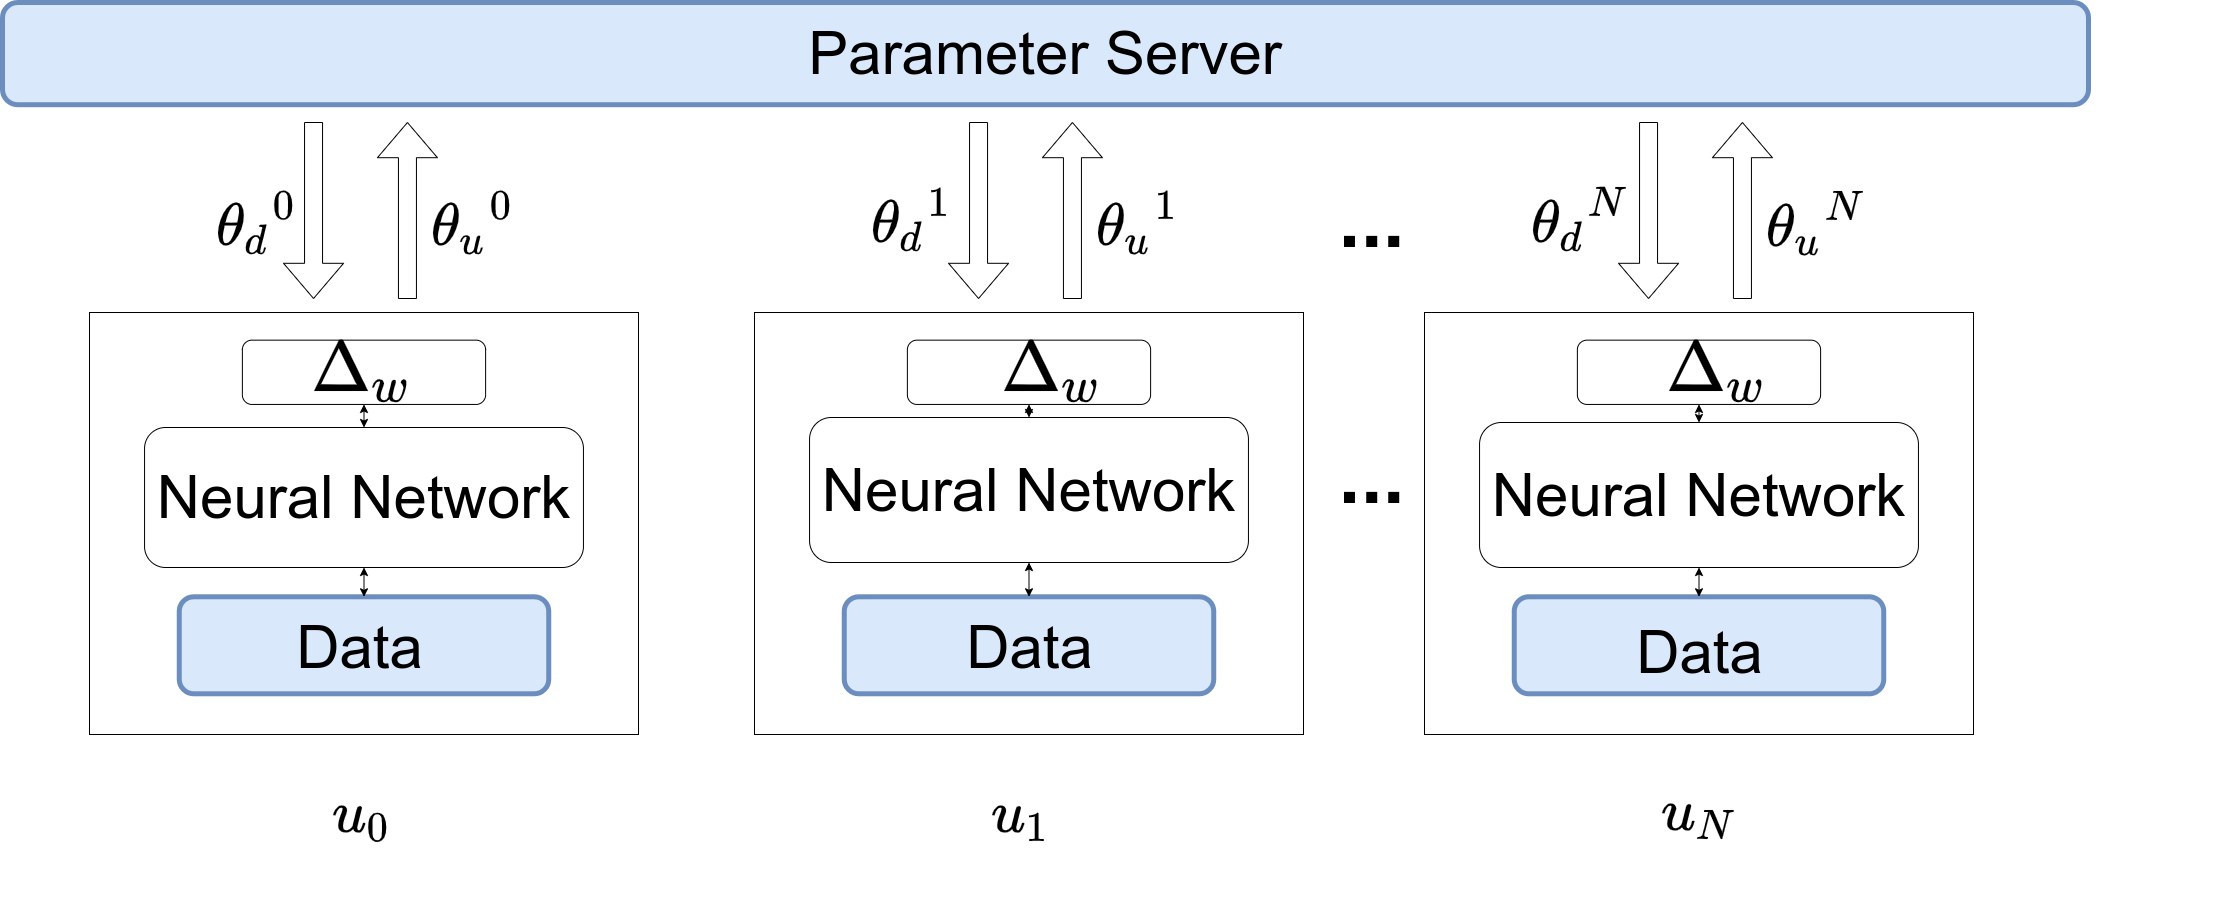
\includegraphics[width=\textwidth, keepaspectratio]{HighLevelArch}
\caption{An architecture for privacy-preserving distributed learning.}
\label{fig:HighLevel}
\end{figure*}
We consider a distributed deep learning system formed by a set of $N$ users $\mathcal{U}= \{u_0, \dots,u_N\}$ and
a parameter server (PS). User $u_0$ aims to train a local deep neural network using its own training data set
$d_{u_0}$ as well as the data sets of the other users $d_{u_i}$. % for all $u_i\in\mathcal{U}\setminus 0$. 
The training data sets $d_{u_i}$'s of all users contain private information that cannot be shared with each other or with the PS.  We
assume the training data set at the reference user is significantly smaller  than the total training data available in the system.
Otherwise, the reference user could achieve a comparable accuracy without having to participate in the distributed learning. 

User $u_0$'s deep neural network is a multilayer perceptron (MLP) as described in Section \ref{sec:MLP} for image classification.
%in a classic feed forward arrangement.
%Each layer in the network is fully connected to the next layer. 
%The networks takes images as its input to its first layer. It then funnels this input through multiple hidden
%layers. An activation function is then applied to the output of each hidden layer. For this network we choose the Rectified Linear Unit
%or ReLU as the activation function. Since this network serves as a classification network, the log soft max activation function is
%applied to the last layer. This results in outputs that are squashed into probabilities that sum to one.  
Fig. \ref{fig:ClassNN} shows the structure of user $u_0$'s MLP for image classification. The network is fed a raw image of  $m
\times m$ pixels. Each pixel is an individual input which is passed through $N$ hidden layers and ReLU activation function with $I$
neurons in each layer. The neural network produces $j$ outputs where each output represents the probability of the image belonging to
the $a_j$th category. Note that although we focus on MLPs for image classification, our results can be easily generalizable to other
architectures and types of data. 
%In a classification network such as this, each output $a_1$ through $a_j$ reflects the probability of the image belonging to that
% class. 
%All outputs pass throughout the softmax layer and therefore sum to 1. 
\begin{figure*}[!h]
\includegraphics[width=\textwidth, keepaspectratio]{ClassificationNN}
\caption{Neural network depicting an image with $m \times m$ pixels fed as input, $j$ outputs  $N$  hidden layers and with $I$ neurons in layer.}
\label{fig:ClassNN}
\end{figure*}

Table \ref{table:1} summarizes the notations used in this work.
\begin{table}[!h]
\centering
\caption{Table1: Summary of notations used in the paper}
\label{table:1}
\begin{tabular}{ | m{0.12\columnwidth} | m{0.8\columnwidth}| } 
\hline
\textbf{Notation} & \textbf{Description} \\
 \hline\hline

$N$ & Number of participants except the system\\
\hline
$u_0$ & Reference User and the  main benefactor of the architecture \\
\hline
$M$ & Mini batch size used for stochastic gradient descent\\
\hline
$\theta_u^{i}$ & Fraction of parameters selected for upload from total available parameters for $i$th user \\
\hline
$\theta_d^{i}$ & Fraction of parameters selected for download from total available parameters for $i$th user\\
\hline
$W_k$ & Weight matrix for layer K in the neural network\\
\hline
$w_i$ & Flattened vector of all parameters in the neural network. \\
\hline
$\Delta w_i$ & Vector of changes in all local parameters due to SGD\\
\hline
$w^{(global)}$ & Flattened parameter vector for server\\
\hline
$E$ & Error function defining the difference between the computed value and expected value of the objective function \\
\hline
$E_i$ & Error function defining...\\% the difference between the computed value and expected value of the objective function \\
\hline
$\alpha$ & Learning rate of the stochastic gradient descent algorithm\\
\hline
$\mathcal{S}_i$ & Set of $\theta_u^{i}$ largest indices selected from $w_i$ \\
\hline
\end{tabular}
\end{table}

%-------------------------------------------------------------------------
\subsection{Privacy-preserving Distributed Learning under the Semi-honest Threat Model}
%-------------------------------------------------------------------------
To allow user $u_0$ to train its deep learning network while preserving the privacy of all users, we could use the distributed
learning approach proposed by Shokri et al. \cite{shokri2015privacy}. 
%This approach allows user $u_0$, as well as the rest of the users,  to use the private data from each other to train a deep learning
% model. 
In the approach proposed in \cite{shokri2015privacy}, each user $u_i\in\mathcal{U}$ trains a local deep learning
network, and uploads certain parameters to the parameter server. The parameter server aggregates the parameters and transmits some of
them back to the users. This iteration can be repeated until the accuracy of the users' deep learning model achieves a minimum value. 
We assume that the architecture and training parameters of  deep neural network that user $u_0$ aims to
train are known  to all other users and the PS.
By only sharing certain parameters of their local models
with a parameter server, it allows them to update their local models without having to transmit any of their samples to each other
from their private sets. 

Specifically, let  $w^{(global)}$ and $w_i$ be the parameters at the parameter server and at user $u_i$, respectively. Let 
$\theta_d^{i}$ and $\theta_u^{i}$ be the percentage of parameters that user $u_i$ downloads and uploads, respectively. Then, 
to initialize the system,  each user $u_i$ randomly sets its parameters $w_i$ to a randomly chosen value and selects a learning rate,
$\alpha_i$. Then, at each iteration,  user $u_i$  downloads $\theta_d^{i} \times |w_i|$ parameters from the parameter server and
overwrites its corresponding parameters, $w_i$, where $|w_i|$ denotes the total number of parameters in $w_i$. User $u_i$ then runs the
stochastic gradient descent algorithm 
with the updated parameter vector as the initial vector. 
Based on the new parameters found by the SGD, i.e., $w_i^{(new)}$, user $u_i$ uses \eqref{eq:SGD} to update its local parameter vector $w_i$. 

Next, user $u_i$ determines which parameters to upload to the server. 
To this end the user first computes 
\begin{align}\label{eq:deltaParam}
\Delta w_i =  w_i^{(new)} -  w_i
\end{align}
which measures the changes between the old and new
local parameters. Then, the user forms set $\mathcal{S}_i$ with the indexes of the elements in vector $\Delta w_i$ that have the top 
$\theta_u^{i} \times |\Delta w_i|$ values, where $|\Delta w_i|$ is the size of $\Delta w_i$. 
The user $u_i$ forms vector $w_{\mathcal{S}_i}$, which contains the parameters in $w_i^{(new)}$ whose indexes are in
set $\mathcal{S}_i$, and uploads it to the parameter server. Note that $w_{\mathcal{S}_i}$  is set to zero in the remaining
positions. 

%$w_i^{(new)}$ with
%that experienced the largest changes.  

%$\theta_u^{i} \times \Delta w_i$ gradient difference values in $\Delta w_i$.  The 

%To determine which parameters to upload, user $u_i$ computes the parameter

After receiving the parameters from user $u_i$, the parameter server updates its own vector as follows:
$$w^{(global)} =  w^{(global)} +  w_{\mathcal{S}_i}$$
%where $\Delta w_S$ is the vector of the largest parameters from user $u_i$. 
Intuitively, by using $w_{\mathcal{S}_i}$, which contains information about the parameters in the local model of $u_i$i that have
undergone the largest changes due to the local SGD training, the parameter server can improve its own parameters that are then
downloaded by other users to further improve their own models.  


Although this approach can train local models with high classification accuracy,  it assumes a semi-honest threat model for the users,
which is not realistic. That is, it assumes that the users will attempt to find private information about other users based on 
the parameters that they download from the server. As we will see in the next section, users can launch active attacks where they
maliciously modify the parameters that they upload to recreate samples from other users. 
%Intuitively,  $\Delta w_i$ measures how much each parameter has to change to more accurately perform classification on the local
%dataset $d_i$.

%trains its local deep neural network using only its local training data set and
%uploads $\theta_u^{i}$
%parameters from its parameter vector $w_i$ to the parameter server. After all users have uploaded their parameters to the server, user
%$u_i$ downloads $\theta_d^{i}$ parameters from the global parameter vector $w^{(global)}$

%The user $u_i$ also choses a value 


%The system also includes a secure parameter server (PS), which
%maintains the latest values of parameters uploaded given by $w^{(global)}$. Each user, $u_i$ in the system selects a 

%Each participant, 
%The participant then 


%In this scenario we assume all participants, $u_0$ to $u_N$, interact with the server atomically.
%That is, at any given time, only one participant can upload or download parameters from the server. This prevents over writing of
%parameters or race conditions from occurring within the server.

%Let $w_i$ be the flattened vector of deep neural
%network parameters for the $i$th user. The deep learning system aims to share parameters of each user $u_0$ to $u_N$  trained privately
%on datasets $d_0$ to $d_N$ in a privacy preserving manner.

%The parameter server is responsible for maintaining the current values of all parameters. Since it should be accessible to all
%participants , the server can be implemented as any form of updatable cloud storage. However, for the purpose of this experiment we
%chose to implement it as another neural network. 




%To train user $u_0$'s model in a privacy 

%However, 

%We assume a reference  participant, $u_0$ whose dataset $d_0$ is significantly smaller
%than datasets $d_1$ to $d_N$ belonging to users $u_o$ to $u_N$. 


%To do this, all participants in this system agree in advance on a common network architecture and common learning objective. 

%---------------------------------------------------------------------------------
\subsection{A Malicious Threat Model for Distributed Deep Learning}\label{sec:threatModel}
%---------------------------------------------------------------------------------

%The main reason to design distributed learning algorithms is to protect the privacy of the users training data sets. 
%This data can be sensitive and an unverified user might attempt to maliciously violate the sharer's privacy on the pretext of model
%training.

In this work, we consider a malicious threat model for both the parameter server and the users. Specifically, malicious users will
attempt to learn private information about other users' dataset based on the parameters that they download from the server. The
parameter server will attempt to learn private information from the parameters that users upload.  In
addition, malicious users upload malicious parameters that can lead a victim user to upload its parameters to the server in such a way
that the malicious users can use them to recreate private data samples from the victim.

%Instead of sharing the parameters of its deep neural, the malicious party will collect the parameters from its victim user. The
%malicious party will then replicate the victim's data, ultimately violating the the victim's privacy.
  
%Such an attack has been  In this attack, 
%Since the threat is not dependent on the
%adversary compromising the
%central Parameter Server, it remains viable. In effect, the adversary does not have to control the PS or the service provider to
%execute his attack. The attack is more effective when adversarial influence is exercised \cite{hitaj2017deep}. This would imply that
%the adversary is an active participant that is adapting his gradients in real time during the current learning process.

%describe an attack that results in privacy leakage in
%collaborative deep learning system proposed in
%\cite{Shokri}.  The attack results in a malicious user inferring sensitive information from a victim's dataset. 

%Specifically, the proposed attack the goal of the  adversary is to extract information from a victim about a class of data he does
%not own. The
%adversary deceives victim into releasing more information about the specific class by presenting himself as an honest participant in
%the collaborative learning  process.    The adversary does launches the
%attack by pretending to be an honest participant and building a local GAN unbeknownst to the other participants.

%The threat model is dependent on an active insider. However, 

%\subsection{Attack Posed}

Such an attack has been described by Hitaj et al. \cite{hitaj2017deep}. In particular, the attack operates as follows. 
Suppose user $u_A\in\mathcal{U}$ is malicious and targets another user $u_V\in\mathcal{U}$. Further assume that all users, including
the malicious one, agree on the hyper parameters of a neural network architecture such as the number, size and type of layers,  and the
classification labels as described in Section \ref{sec:systemModel}.

The victim user $u_V$ declares that its private training data set contains samples for the  labels $[a,b]$. The adversary
$u_A$ declares to have the classification labels $[b,c]$ in its training data set, which means it has no data for label $a$. By
deploying the attack, the adversary aims to replicate samples with the same probability distributions as the private samples with label
$a$ at user $u_V$.

The adversary user $u_A$ then locally uses a generative adversarial network to generate samples that have the same distribution as
sample with label $a$ at $u_V$. The adversary labels these malicious samples as belonging to category $c$. This prompts the victim 
user $u_V$ to share \hl{more revealing parameters [How exactly?]} which results in more information about
its samples in class $a$ being revealed to the parameter server. Ultimately, the adversary $u_A$ can access the more revealing
parameters from $u_V$ by downloading parameters from the server. 
%classes
%$a$ and $c$. Therefore the victim releases more data on class a now than he initially intended to.

We summarize the attack proposed by \cite{hitaj2017deep} as follows \hl{[Usae algorithmic environment for this summary. Can be done
later]}:
\begin {enumerate}
\item Assume victim $u_V$ declares labels $[a,b]$ and adversary $u_A$ declares labels $[b,c]$
\item Run the distributed deep learning protocol proposed by \cite{shokri2015privacy} for several epochs and stop when we reach a
specified accuracy.
\item During this process, the $u_V$ downloads a percentage  of parameters, $\theta^V_d$ ,  from the
parameter
server and updates his local model.
\item $u_V$'s local model is trained on classes $a$ and $b$
\item $u_V$ uploads a section of his model to Parameter Server
\item The adversary training is slotted to engage with the Parameter Server
\item $u_A$ downloads the percentage of parameters, $\theta^A_d$ , from the PS and updates its model
\item $u_A$ then trains its local GAN to generate samples with the same distribution as class $a$ at $u_V$.
\item $u_A$  mislabels class $a$ samples as class $c$ samples.
\item $u_A$ uploads a percentage of its parameters, $\theta^A_u$, to the PS
\end {enumerate}

%During the process of convergence, $u_A$ will be able to covertly exert influence on the learning process via the mislabeling of class
%$a$.

In this work, we present a collaborative learning scenario that prevents the malicious user from recreating private sample
from other users. 

%releasing more
%information about a class, and ultimately it protects the reference user's privacy. We design the interaction of the reference user
%with Parameter Server such that $u_V$ is not RefU


%---------------------------------------------------------------------------------------
\section{A Privacy-preserving Distributed Learning Algorithm}
%---------------------------------------------------------------------------------------
\begin{figure*}[t]
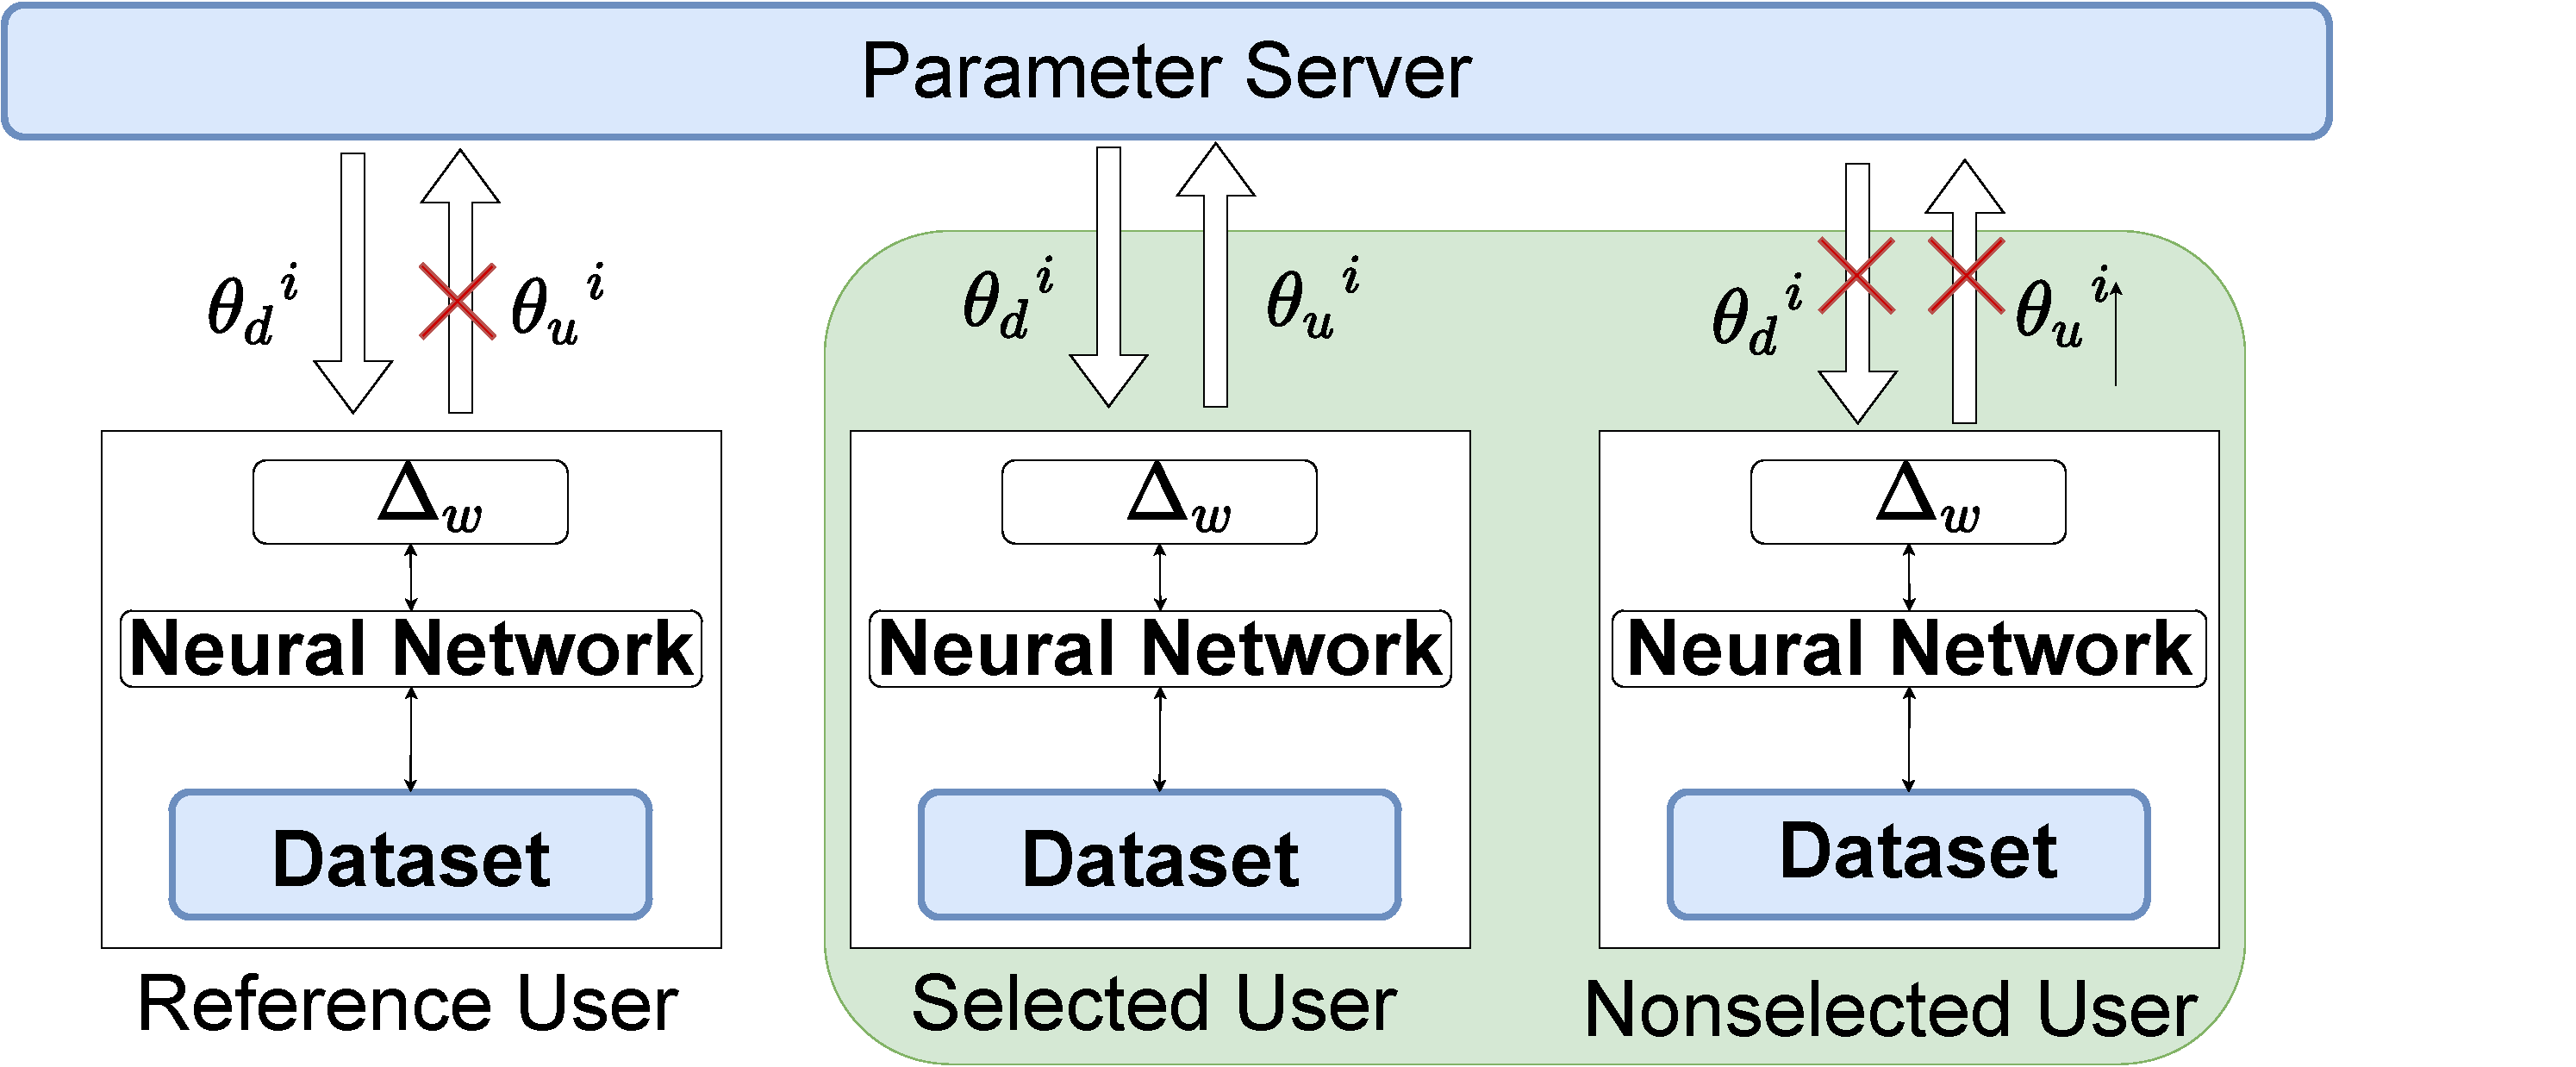
\includegraphics[width=\textwidth, keepaspectratio]{OurHighLevelApproach}
\caption{One iteration of our proposed algorithm for privacy-preserving distributed learning.}
\label{fig:HighLevel}
\end{figure*}
In this section we describe our proposed privacy-preserving distributed learning algorithm, which prevents attacks
such as the ones described in Section \ref{sec:threatModel}. Instead of attempting to protect the privacy of all users as in 
\cite{shokri2015privacy}, we instead focus on protecting the privacy of a single users, called the reference users as described in
Section \ref{sec:systemModel}. Our main approach to protect the reference user's privacy is to prohibit the reference user
from uploading its parameters to the  parameter server. 

Although we focus on the privacy of the reference user, our approach also
limits the amount of private data that other users expose to an attack. To protect the rest of the users, out algorithm only allows
them to upload and download parameters from the server a limited number of times and in random order. 
This randomized choosing of participants reduces the chances of selecting the malicious participant in every round, limiting
the adversary's ability to upload malicious parameters that can force other users to reveal private data. 
This is in contrast to \cite{shokri2015privacy} where all users participate during all iterations. 
%Our proposed algorithm prevents attacks such as the one proposed in \cite{hitaj2017deep}. 

%Specifically, we protect the participants from GAN based attacks by preventing an innocent user from parameter sharing in a
%predictable and repeated way which reduces the adversarial influence as described in \cite{hitaj2017deep}.  We randomly choose the set
%jof
%participants that can interact with the server at one time period called the round, $r$.  

Our approach works as follows. 
%We suppose all participants in the architecture agree on the hyper parameters such as
%classification labels, type and architecture of neural networks. All participants data sets from all users are considered private
%information that needs to be protected from other users and the parameter server. 
We assume a user $u_0$ who aims to train a local deep neural network using its local training data set as well as the training
data sets from other users as described in Section \ref{sec:systemModel}.  We then form set $\hat{\mathcal{{U}}}$ by randomly selecting
users from set $\mathcal{U}$. The reference user is never chosen.  
%such that only one participant interacts with the server at one time. 
User $u_i\in\hat{\mathcal{U}}$ downloads a fraction $\theta_d^i$ of the parameters
in the server, and uses them to overwrite its  corresponding local parameters in $w_i$.
User $u_i$ then trains its network privately using its local data set  $d_i$, and obtains the new parameters $w_i^{(new)}$.
Then, as described in \eqref{eq:deltaParam}, user $u_i$ calculates the change in parameter values by computing $\Delta w_i$, groups the
indexes of the elements in vector $\Delta w_i$ with the largest $\theta_u^i\times |\Delta w_i|$ values in set $\mathcal{S}_i$, and 
forms a vector $w_{\mathcal{S}_i}$ with the elements in $w_i^{(new)}$ that correspond to indexes in $\mathcal{S}_i$. 
User $u_i$ uploads $w_{\mathcal{S}_i}$ to the parameter server who aggregates them. 

%before the next selected participant can interact with the server. 
After all selected users in $\hat{\mathcal{U}}$ have uploaded their parameters, reference user $u_0$ downloads the aggregated
parameters from the server. It then uses the downloaded parameters as initial parameters to retrain its local model. 

Note that the reference user  $u_0$ never uploads its parameters to the server, and thus its private data is protected from the
parameter server and other users. 

%Also, note that the selected users in $\hat{\mathcal{U}}$ download the parameters from the server,
%train their network, and upload their parameters only during one epoch. 

We summarize our proposed algorithm as follows:
\begin {enumerate}
\item Out of all available participants, a random subsection of participants is selected to interact with the parameter server in this
period. We call this period a round which is denoted by $r$. In each round, $r_i$, the selected users are able to interact with the parameter exclusively such that no two
participants can interact with the parameter server at the same time.
\item During its interaction with parameter server, a selected user $u_i$ will perform the following steps:
\begin {enumerate}
  \item Train independently on its local dataset for one epoch, to calculate parameter gradient, $\Delta w_i$ 
  \item  At the end of the epoch, $u_i$ will select the $\theta_u$ fraction of highest gradients in its local $\Delta w$. It will then upload that fraction of values in $\Delta w_i$ to the parameter server.
  \end {enumerate}
\item For each subsequent epoch, the participant will first download $\theta_d$ percentage of parameters from the server. The
user will then repeat the steps a and b. We repeat these steps for every participant selected in $r_i$.
\item At the end of $r_i$, the reference user downloads $\theta_d$ percentage of parameters from the parameter server.
\item The reference user, $u_0$, then trains its model locally on its dataset. 
\end {enumerate}

%As you can see the, the reference user does not share its parameters with other users. It benefits from random particpants from the
%architecture but does not expose itself to any attacks. Since the participants selected from the pool each round are randomized, we ..



%-------------------------------------------------------------------------------
\section{Experimental Results}
%-------------------------------------------------------------------------------

To evaluate the performance of our proposed privacy-preserving approach, we implement it on a commercial cloud service provider, and
measure the learning performance of the user $u_0$, and compare it to the learning performance of a centralized deep neural network
architecture, and to the distributed learning architecture proposed by Shokri et al. \cite{shokri2015privacy}. 
%without collaborative
%learning.
%We wrote the source code based on the pseudocode provided in paper \cite{Shokri}. 

%----------------------------------------------------------------------------
\subsection{Experiment Setup}
%------------------------------------------------------------------------------
We implement all algorithms using Torch with the neural network packages in the scripting language LUAJIT, and run them on an M4
instance on the Amazon Web Service's Elastic Compute Cloud (AWS EC2), which has
2.4 GHz Intel Xeon E5-2676 v3** Processor, 4 VCPUS and 16 GB RAM.
\begin{figure*}[t]
\centering
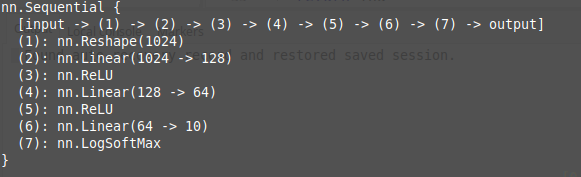
\includegraphics[width = 2 \columnwidth, keepaspectratio]{MLPArchitecture}
\caption{MLP architecture displaying the tensor size at various stages in the neural network. }
\label{fig:MLPArch}
\end{figure*}
As described in Section \ref{sec:systemModel}, we use a 
% implement a similar neural network structure for the reference user as well as
%other participants.
%Although one can chose any neural network architecture, 
a multilayer perceptron (MLP) in a feed forward arrangement. To train it, we use the MINST training data set \cite{deng2012mnist}, which contains 
$32\times 32$ pixel images of handwritten numbers. Accordingly, our MLP has 1024 input nodes
corresponding to each pixel in the images, and the output layer is a tensor of size 10 where each output corresponds to the probability
that a given input is a specific number
between 0 and 9.  The model has 2 hidden layers where the non-linear ReLU activation function is applied to the
output of each hidden layer.  The first hidden layers are constructed via \textit{nn.Linear()} which applies a linear transformation
and produces a tensor of size 128 as its output. The second hidden layer accepts a tensor of size 128 as input, and outputs a tensor of
size 64.The last layer of the model is a log soft max layer implemented by the \textit{nn.LogSoftMax()} module.  This activation
function is usually applied to the end of all classification models where it squashes the inputs into probabilities that sum to one.
The architecture of the MLP used in our experiments is illustrated in Figure\ref{fig:MLPArch}.



%We conduct our experiments with varying number of users, 
%fraction of upload gradient $\theta_u$, probability of interaction with Parameter Server and number of rounds of training $r$.

%We were able to replicate their original setup using
%Torch and nn packages in LUAJIT scripting language.  
%The tests on the proposed solution were run and hosted 


%We used the MLP implementation of neural network using the function \textit{nn.Sequential} container via the Torch nn package. They are
%fully connected and the neural network has input data of size 1024 (32 x 32) and feed fowards

%-------------------------------------------------------------------------------
\subsection{Datasets}
%-------------------------------------------------------------------------------
We conducted our experiments using the MNIST dataset \cite{deng2012mnist}. The MNIST dataset is a standard dataset used in image
recognition. It contains images of hand-written gray scale digits ranging from 0 to 9. The dimension of each image is 32 X 32 pixels.
The MINST dataset contains 60,000 images in its training dataset and 10,000 images in its test dataset.
For this experiment, we center the images through a normalization operation.  

We set the size of the local dataset of each participant to 1 \% of the training dataset images.  The Reference User starts with a
training set of 60 images.


%--------------------------------------------------------------------------------------------
\subsection{Hyper-parameter Setup}

%--------------------------------------------------------------------------------------------

Hyper-parameters are parameters that control the collaborative learning process, e.g., learning rate $\alpha_i$, fraction of upload and
download gradients $\theta^i_u$ and $\theta^i_d$ respectively. Unlike the deep neural network parameters that are obtained through
training, hyper parameters are usually set beforehand and remain constant through out the training and inference phases. They are
crucial since they directly influence the behavior of training algorithm and have a large impact on the performance and accuracy of the
model. In our experiments, we set the learning rate $\alpha_i$ for all users to $0.1$.  The mini-batch size $M$ for stochastic gradient
descent training is set to 10 samples.

 
 %We vary the $\theta_u$ and epochs in differentcenarios. 




%--------------------------------------------------------------------------------------------
%\subsection{Framework}
%---------------------------------------------------------------------------------------------

%We conduct our experiment within the Torch 7 and Torch 7 nn framework. Torch is a popular framework utilized for deep learning by major
%software companies. The code for the experiment is written in LuaJIT which is a scripting language based on Lua.  We deploy our
%architectural framework with multiple neural networks on the AWS EC-2 machine to leverage greater processing speed.

%-------------------------------------------------------------------------------
\section{Experiment Results}
%-------------------------------------------------------------------------------

\begin{figure}[!h]
\centering
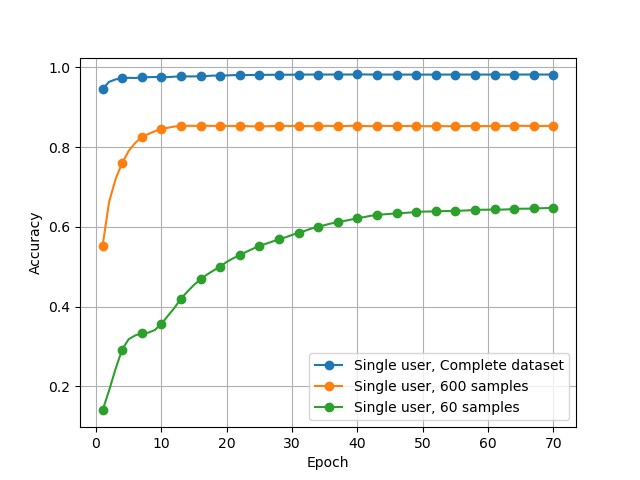
\includegraphics[width=\columnwidth, keepaspectratio]{SingleUserBaselinesGrid}
\caption{Single User with varying sample size.}
\label{fig:SingleUser}
\end{figure}
To fairly assess the performance improvements offered by our proposed privacy-preserving algorithm, we first measure the accuracy of
the centralized approach, i.e., a single entity who collects the data from all users but does not provide privacy. 
Figure \ref{fig:SingleUser} shows the accuracy of the centralized approach for a varying number of epochs. As expected, we see that
that the accuracy obtained by the centralized approach increases with the number of epochs. 
Moreover, to assess the impact of users who only have access to their local data set and do not participate in distributed
learning, we measure the accuracy for different sizes of the training data set. We see that the accuracy decreases with the number
of samples in the data set. This confirms that a small local data set can only provide a low accuracy to the reference user $u_0$.
%We also observe that the accuracy can increase when we use a larger proportion of the data set during training. 
%on a larger
%dataset has a higher accuracy. The user with the highest accuracy has had access to the complete MNIST training dataset of 60,000 samples. 


\begin{figure}[!h]
\centering
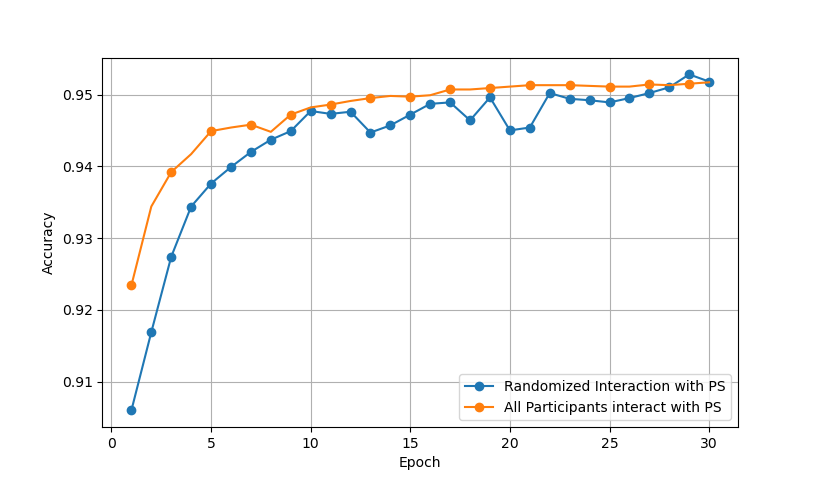
\includegraphics[width=\columnwidth, keepaspectratio]{RandomVsAllGrid}
\caption{Comparison between randomized interaction and complete interaction with server. }
\label{fig:RandVsAll}
\end{figure}

We also tested with a scenario in which all participants simply uploaded their local parameters to the server without downloading any parameters. Only the reference user was able to download the parameters from the server. In this case, $\theta_d^i$ was 0 for every participant except the reference user.
\begin{figure}[!h]
\centering
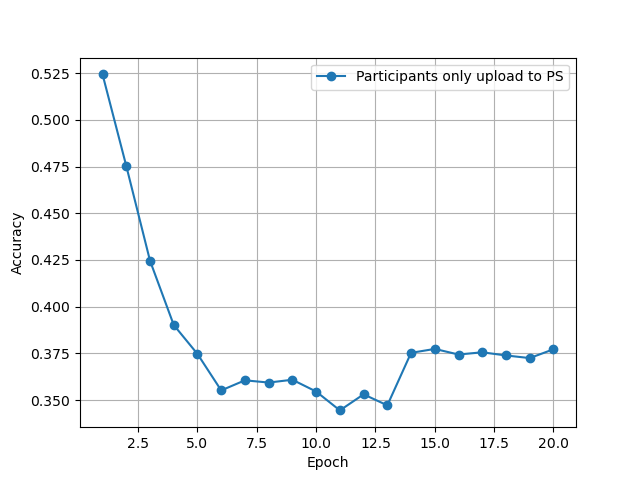
\includegraphics[width=\columnwidth, keepaspectratio]{AllUploadNoDownloadGrid}
\caption{Accuracy of reference user when all participants simply upload parameters to server. }
\label{fig:AllUploadNoDownloadGrid}
\end{figure}


This approach did not show great results. Figure \ref{fig:AllUploadNoDownloadGrid} shows the accuracy of the reference user is negatively impacted in this scenario with each epoch. This shows that downloading the parameters from the server and performing local training is a crucial aspect for the efficacy of this architecture.

Next, we compare the accuracy of the reference user under our proposed privacy-preserving algorithm and that of the algorithm proposed
by Shokri et al. \cite{shokri2015privacy}. Figure \ref{fig:RandVsAll} shows the accuracy of the reference user $u_0$'s deep learning
neural network trained under our proposed deep learning algorithm, and under \cite{shokri2015privacy}. We set the number of
users to 20 for both approaches. In our approach, each of the non-reference users $u_i$ is randomly
selected to upload and download parameters from the parameter server with a probability of 0.5. 
In the approach by \cite{shokri2015privacy}, all users upload and download with a probability of 1. 
We see that the reference user $u_0$ is able to obtain a deep learning model with an accuracy that is comparable to the one
obtained by \cite{shokri2015privacy}, which is vulnerable to the attack in \cite{hitaj2017deep}. 

\begin{figure}[!h]
\centering
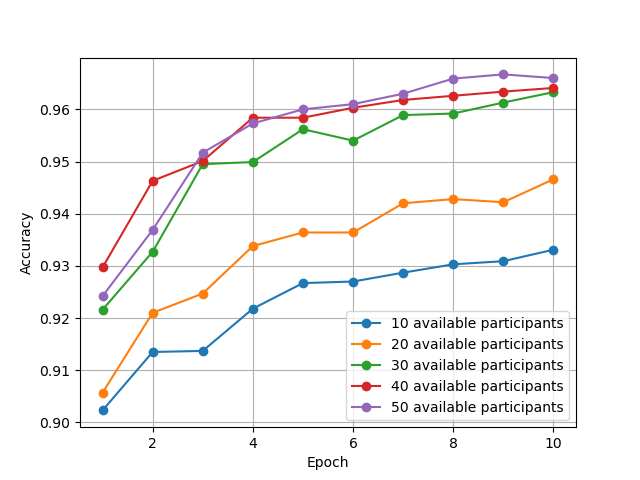
\includegraphics[width=\columnwidth, keepaspectratio]{VaryingPoolofParticipantsGrid}
\caption{Accuracy of Distributed SGD for varying participants available for interaction with the PS.}
\label{fig:VaryingPoolofParticipants}
\end{figure}

Figure \ref{fig:VaryingPoolofParticipants} shows the accuracy of the reference users $u_0$'s deep neural network under a varying number
of epochs for different numbers of total users in the system. We observe that  the reference user $u_0$ achieves a higher accuracy as
the total number of participants in the system increases. For example, the highest accuracy is achieved with 50 participants, while the
lowest one is achieved with 10 participants. This means the parameters uploaded to the server increases with the number of users, improving the accuracy of the
model. The reason is that a larger  number of participants brings a larger and more diverse dataset. 

\begin{figure}[!h]
\centering
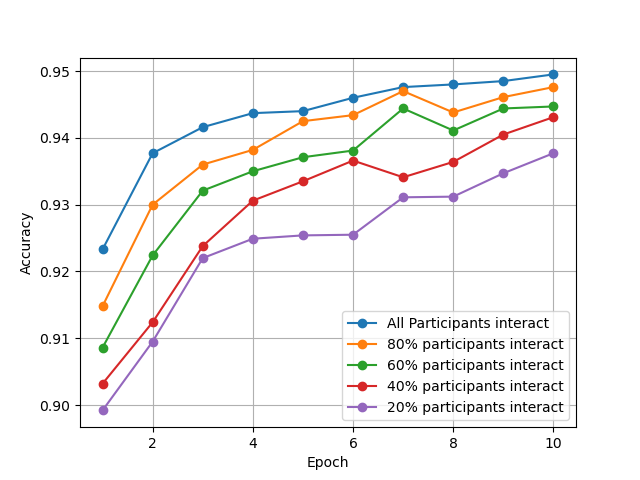
\includegraphics[width=\columnwidth, keepaspectratio]{VaryingProbabilityInteractionGrid}
\caption{Accuracy of Distributed SGD for varying probability of interaction with the PS. }
\label{fig:VaryingProbabilityInteraction}
\end{figure}

Figure \ref{fig:VaryingProbabilityInteraction} shows the accuracy of reference user $u_0$ for a varying number of epochs under
different probabilities for the users to interact with the parameter server. 
We see that a greater probability of interaction with the server results in a higher model accuracy for the reference user $u_0$.
The highest accuracy is obtained when all participants interact with the parameter server. However, this is equivalent to the
approach proposed by \cite{shokri2015privacy} and thus it is vulnerable to the attacks described in \cite{hitaj2017deep}. 

%is in close
%proximity to
%accuracy yielded by models with lesser
%probabilities
%of interaction with PS. 
%Over several epoch the lines representing randomized interaction reflect a smooth convergence.

\begin{figure}[!h]
\centering
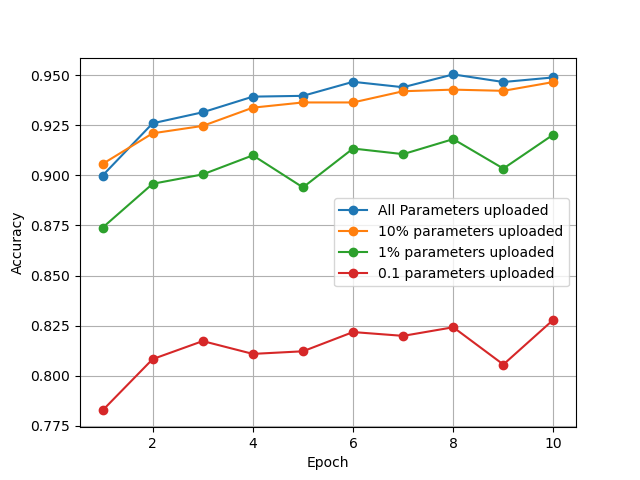
\includegraphics[width=\columnwidth, keepaspectratio]{VaryingThetaUGrid}
\caption{Accuracy of Distributed SGD for different upload gradient selection rate. }
\label{fig:VaryingThetaU}
\end{figure}

Figure \ref{fig:VaryingThetaU} we plot the accuracy of the reference user $u_0$ for different upload gradient selection rate over. 
The plot shows that the percentage of uploaded parameters, $\theta_u$, is directly proportional to the resulting accuracy of
the model at $u_0$. However, the accuracy difference between the sharing all parameters and only $ 10\% $ percent of parameters is
insignificant.



%-------------------------------------------------------------
\section{Conclusion}
%------------------------------------------------------------

In this work we design, implement and analyze a secure privacy preserving approach to distributed deep learning systems.  Our
algorithm provides security against attacks that extract information from participants in a collaborative setting. 

Our work can be extremely beneficial in providing a secure application of distributed and decentralized collaborative learning. This
will make it more accessible to users concerned about their privacy but want to benefit from larger datasets.

Our methodology provides countermeasure to the category of attacks that use malicious parameters to influence victims to reveal more
information as described  by Hitaj  et al. \cite{hitaj2017deep} . We do this by limiting the consistent exposure of each participant to
the server and to other users. Our solution does not rely on computationally expensive cryptographic process and has a adaptable
architecture that can be used with any underlying neural network structure. For the scope of this work we assume that the multiple
users and the parameters are non-colluding and only share information outlined by our protocol. 

Our experiments show that ... \hl{main result}. 
\bibliographystyle{IEEEtran}
\bibliography{references}


\end{document}